\documentclass[12pt]{article}
%Gummi|065|=)

\usepackage{fancyhdr}
\usepackage{listings}
\usepackage{graphicx}

\graphicspath{ {testing/}{design/} }
\pagestyle{fancy}
\title{\textbf{CS12320 - Main Assignment\\
				Bonks and Zaps}}
\author{Josh Smith\\
		jos67@aber.ac.uk}
\rfoot{\tiny{Document compiled on \today}}
\date{}
\usepackage{amsmath}
\begin{document}


\maketitle
\newpage

\tableofcontents

\newpage


\section{Introduction}
For this write-up I will be walking through some of the choices I made throughout my assignment. I will mainly focus on the decisions related to the structure of my classes; some of these main decisions will be choice of classes and uses of inheritance throughout the project.

\section{Design}
This section will contain the portions of my write-up regarding the design of my assignment.

\subsection{Class Diagam}
The class diagram can be found on the next page due to sizing issues. If the diagram is still too small, you can find an SVG of the UML diagram inside the zip file.
\begin{figure}[hpc]
	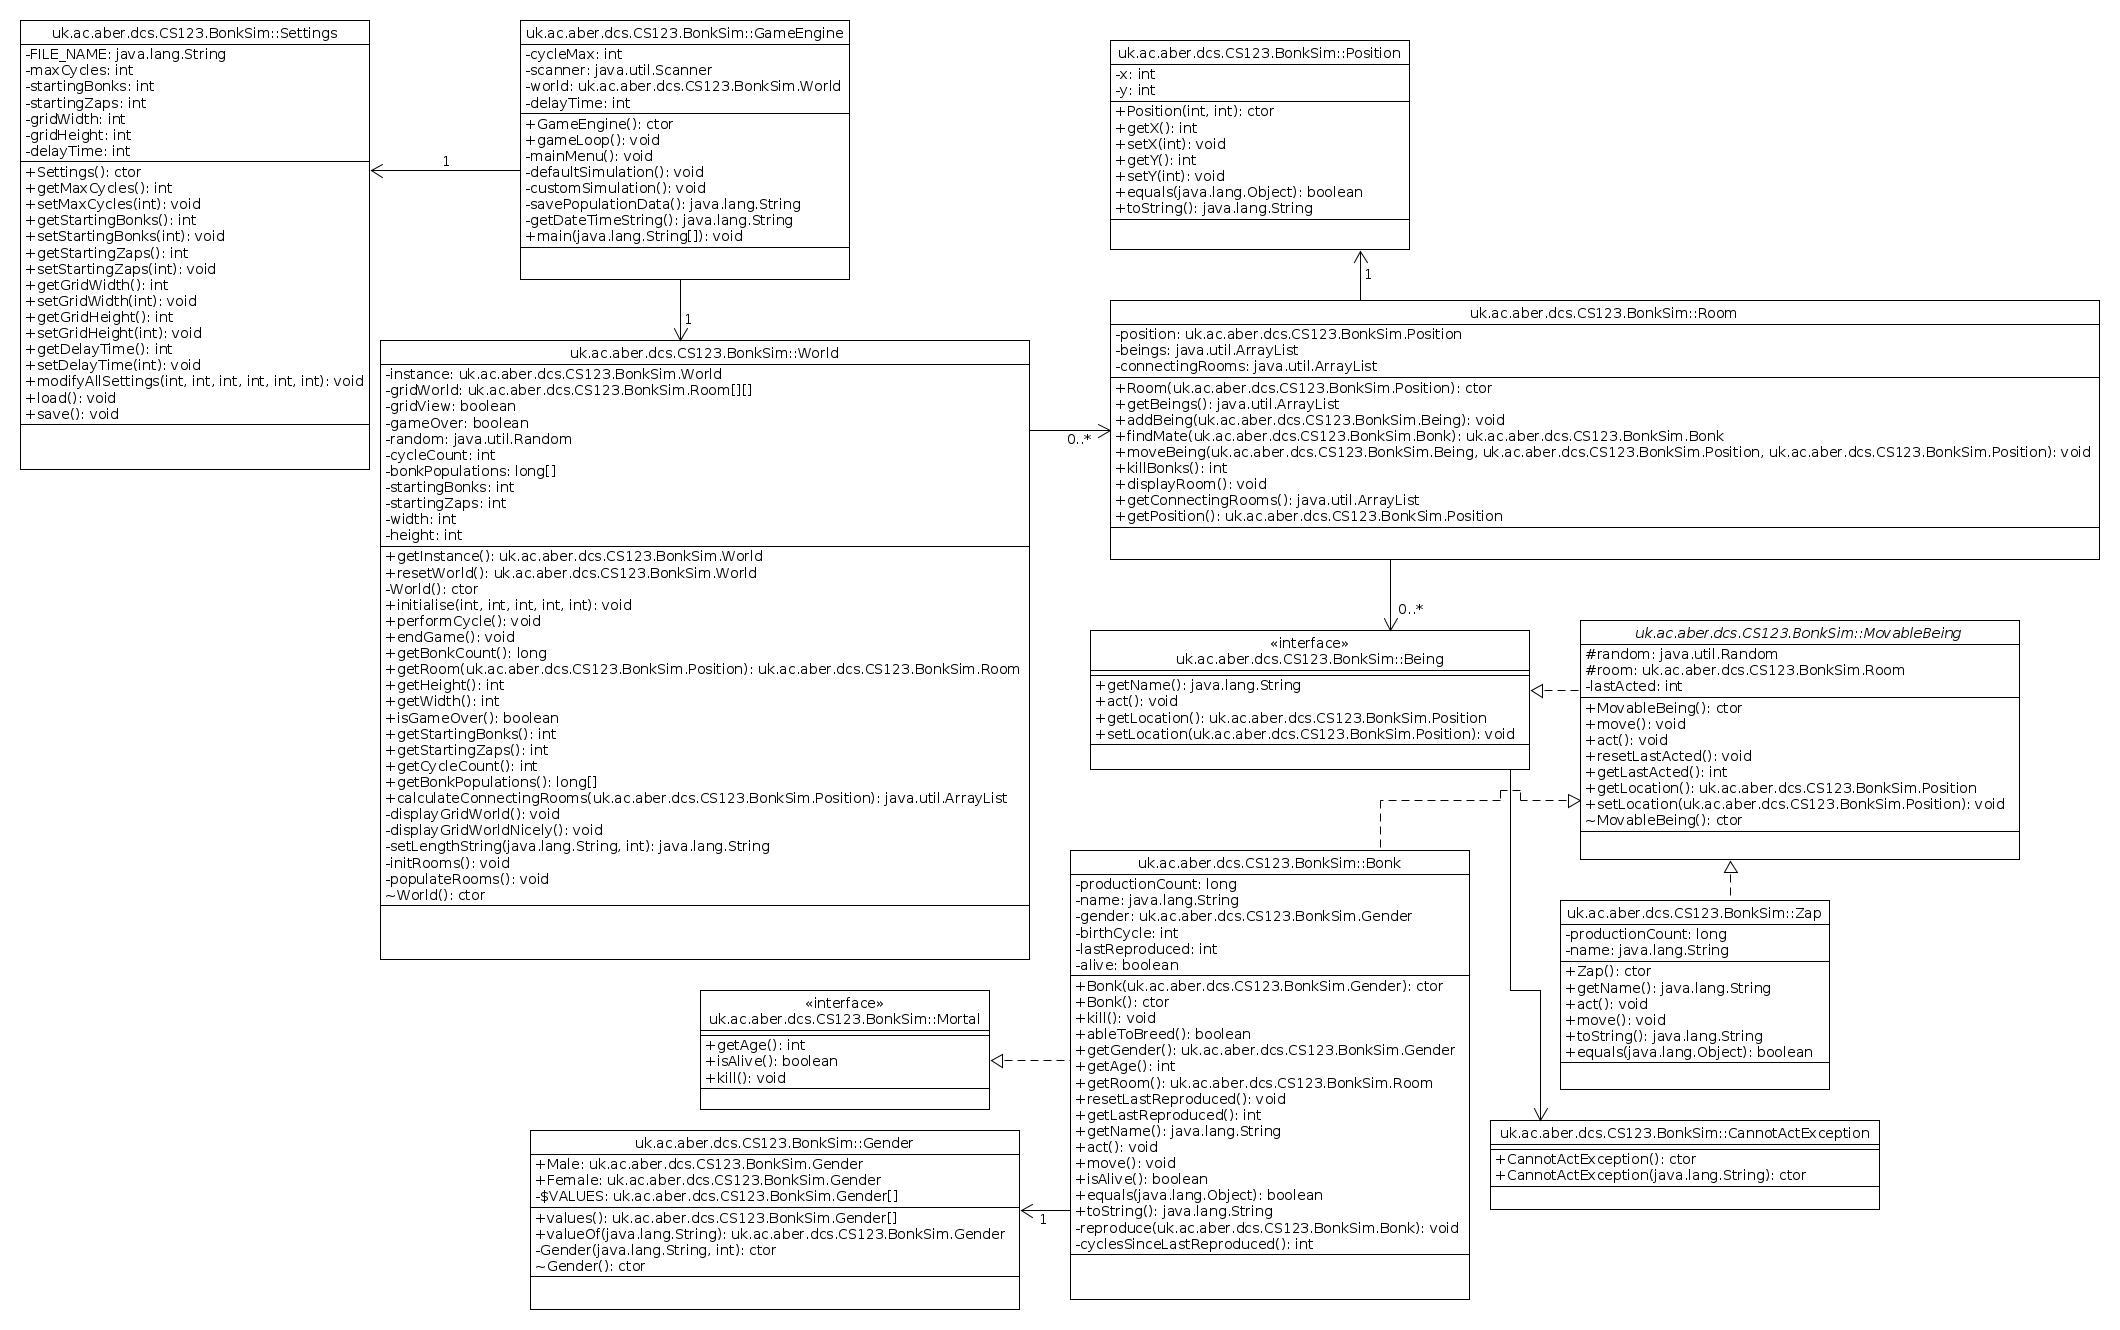
\includegraphics[width=\paperwidth,angle=90]{UML}
\end{figure}
\newpage
\subsection{Class Descriptions}
This section is going to consist of a textual breakdown of each class and its primary functions.

\subsubsection{GameEngine}
The main purpose of this class is to perform the primary operations of the 'game', these operations include:
\begin{itemize}
	\item Running the main game loop.
	\item Displaying the menu.
	\item Managing general data about the game.
\end{itemize}
The game engine also manages the initialisation of the world to be used for the 'game'. I decided to keep the GameEngine class as bare bones as possible to allow for possible alternate worlds to be added with ease. \\

\begin{lstlisting}[caption=Game loop, basicstyle=\small]
do
	world.performCycle
	delay
until gameOver OR (cycleCount == maxCycles)
\end{lstlisting}

This means that most of the decisions are made by the world object and any logic within the performCycle() function.

\subsubsection{World}
This class is used as the main component for the 'game' as it performs the main operations such as displaying the grid and iterating through the grid to tell every being within a room to perform its act() method. \\

I decided to implement the class with a singleton. This means that a world object cannot be instantiated from outside the class and is stored within a static variable. This allows me to have a single instance of World used throughout the 'game' which can be easily accessed by other classes through the World.getInstance() function. I chose  to implement it this way as I only intended for a single world to be in use at one time.\\

The class also manages the grid which is implemented as a two-dimensional array of Room's (See 2.2.3 for info on the Room class). In the brief the grid system was defined to have set movements beings can take from one room to another, to implement this I created a function within my world class called calculateConnectingRooms() which is used by the Room class inside of the constructor to tell each room which rooms it is 'connected' to.

\begin{lstlisting}[language=Java, basicstyle=\tiny, caption=performCycle function]
    public void performCycle() {
        // gameOver is always true unless a living bonk is found.
        gameOver = true;
        long bonkCount = getBonkCount();
        bonkPopulations[cycleCount] = bonkCount;
        System.out.println("Cycle: " + cycleCount + " - BonkCount: " + bonkCount);
        for (Room[] col : gridWorld) {
            for (Room r : col) {
                // Creates a copy of the list for us to iterate through despite
                // modifications during b.act()
                ArrayList<Being> beings = new ArrayList<>(r.getBeings());
                for (Being b : beings) {
                    if (b instanceof Bonk) {
                        if (((Bonk) b).isAlive()) {
                            gameOver = false;
                        }
                    }
                    try {
                        b.act();
                    } catch (CannotActException e) {
                        System.err.println("ERROR: Cannnot act.");
                    }
                }
            }
        }
\end{lstlisting}

This function takes care of everything that needs to be done for a singular game cycle within the world. \\

I chose to draw the world at the end of a cycle rather than the start of a cycle so that it shows the state of the grid world after any changes have been made. The grid is drawn through a seperate function named displayGridWorldNicely() as this is the successor to the initial function I had during the start of my project when I wanted to quickly see if things were changing without having to write out an aesthetically pleasing terminal UI. I opted against a JavaFX based UI for the grid world as this would have taken me a lot longer and I was happy with my terminal output.\\

Throughout each cycle I am collecting data within the bonkPopulations variable which is of type long[] as this allows me to graphically display the changes in bonk populations for each cycle (More in section 2.2.9).

\subsubsection{Room}
This class plays a very key role within the 'game' as it acts as a container for the Beings at its 'location' within the array. The location is relative to the index of the room within the two-dimensional array of Room's within stored World.\\

The class also keeps a list of rooms which it is 'connected' to as mentioned earlier in the section 2.2.2. These connecting rooms are used when a being is performing its move logic (See section 2.2.4). The constructor for Room takes a Position (See 2.2.5) as this allows it to know its place in the world and request information from the World such as which rooms are connected to it.\\

The room stores the beings in a single list rather than separating them by type as this helps maintain balance with the bonks/zaps acting in an order defined by their position in the list; this is a first in first out approach. The room class will also have a major job in the bonk reproduction process as it will be used to find potential mates for the bonks every cycle. The function findMate() shall be called from within the Bonk class and will check the list of beings for any bonks which are of the opposite gender and are eligible to breed this cycle. Eligibility to breed is defined in the brief as a bonk which is more than one cycle old and has not been involved in any other reproduction this cycle. To prevent this I am storing the current cycle in a variable called lastReproduced whenever the bonk reproduces and then comparing it with the current cycle to check its eligibility.  

\subsubsection{MovableBeing}
This class is an abstract class as it should never be used on its own. This class is mainly used to prevent code duplication and make use of inheritance. Both bonks and zaps are types of MovableBeings and therefore both inherit from the class. The main function this class contains is the move() functions which has the logic for random movement based on connecting rooms. I am using a static random variable rather than instantiating a new random each time the move() function is called as the java Random class uses time in milliseconds as a seed which could call issues if two Randoms are instantiated within a single millisecond which would not be unreasonable. \\

This class also implements the Being interface we were given in the brief and implements the methods getLocation() and setLocation() in a slightly roundabout way. Because of my approach to the problem (using a two dimensional array of rooms) I chose to have the setLocation() function simply ask the world for the room at the location passed based on an index of Position.getX() and Position.getY().\\

For my act() function I am ensuring that before anything is done that the being meets certain criteria. It is vital that the being is aware of the last cycle that it acted as if the being moves to another room before that room has had its cycle then the being will act again. To prevent this I am checking that the lastActed variable is not the same as the current cycle. I am also checking that the being is alive before allowing it to act. 
\subsubsection{Position}
This is a very simple class implemented to work with the interface provided. It has an X and a Y value with functions to get the values.
\subsubsection{Bonk}
This is the first of the two Beings in use in the current state of the 'game'. Bonks inherit from MovableBeing and also implement the Mortal interface (See 2.2.8). Due to the specification bonks are implemented with a set Gender (see 2.2.9), this only makes a difference during reproduction. For my naming convention I chose a simple format of the letter B followed by the number which uniquely identifies the Bonk (The number of bonks produced so far this 'game' at the time of instantiation). I have a function implemented called ableToBreed() which returns true if the bonk meets all the criteria needed to reproduce this cycle; this helps reduce code duplication and ensures that I only have to change this one function if any changes are made to the criteria.

\subsubsection{Zap}
This is the second of the two beings currently in use. Zaps also inherit from MoveableBeing however do not implement the Mortal interface as they cannot die. Zaps are a very simple being as they do not have the reproduction mechanic. As specified by the brief the only task for the zap is to kill all of the bonks within its room every time it is called upon to act which is once per cycle. The zap also has its own static productionCount variable for uniquely identifying the zaps; they follow a similar naming convention to bonks however I use a Z followed by the productionCount at the time of instantiation.
\subsubsection{Mortal}
This interface is simple and could possibly be considered unnecessary but since the brief mentioned that there is a likelyhood that more mortal beings will be added in the future, this allows for less code duplication throughout these other mortal beings.\\

This interface ensures that the classes which implement it have a getAge() function, an isAlive() function and a kill() function. These are the three key components to being a mortal.

\subsubsection{Settings}
This class holds all of my settings for custom simulations. The individual settings are stored as static variables and can be saved/loaded by using the static save/load functions. Any of the settings can be accessed using Settings.<SETTING>.
  
\section{Testing}
Disclaimer: All testing was done on a Linux system running Fedora 23 using Oracles Java version 8.

\subsection{Test 1}
This test ensures that the 'game' ends after the specified number of cycles.

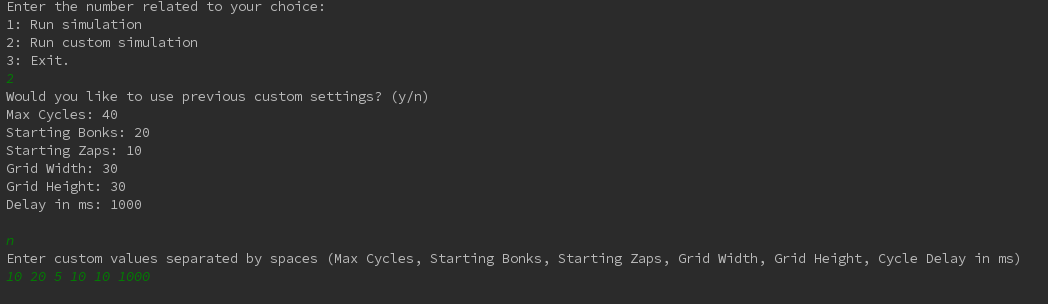
\includegraphics[width=15cm]{test1a}
As you can see the settings are entered to set the game to run for 10 cycles.\\
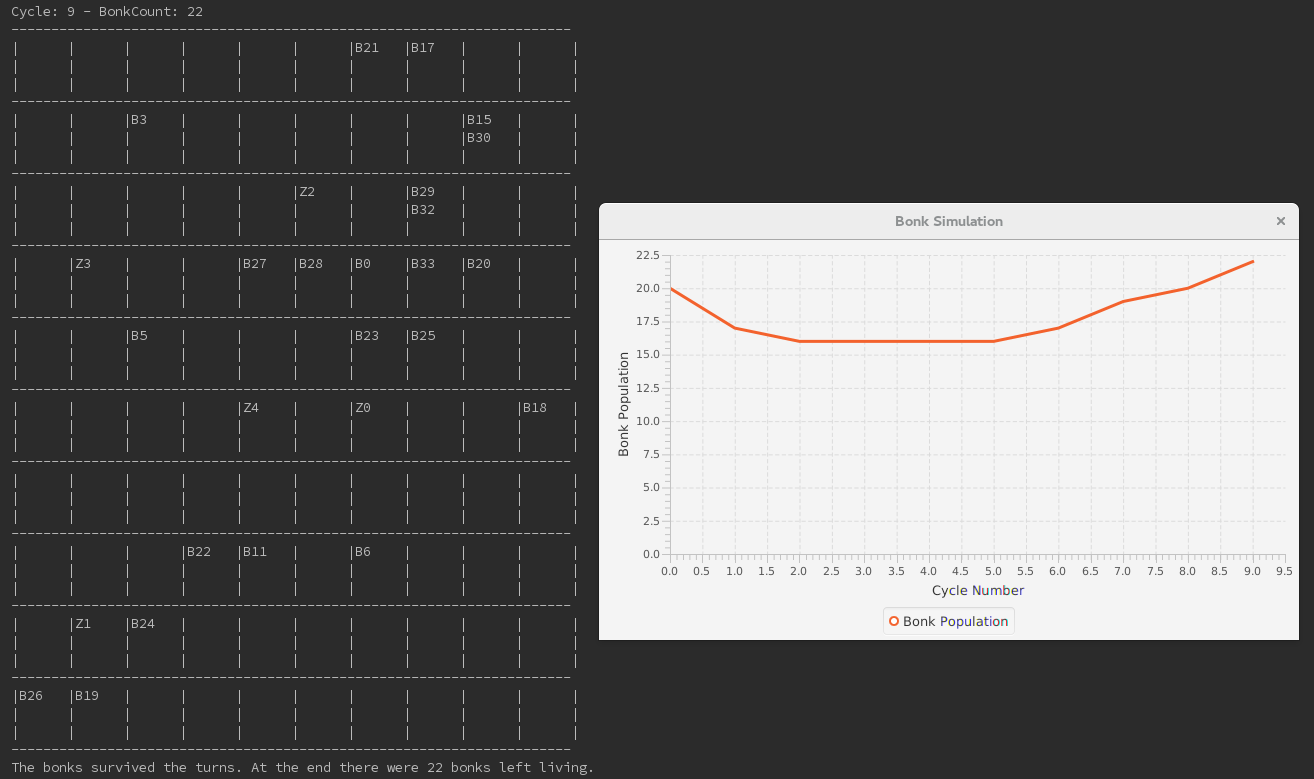
\includegraphics[width=15cm]{test1b}
The bonks survive the turns after cycle 9 (cycle 0 is the first cycle therefore cycle 9 is the 10th cycle) The game performs as expected and the graph is shown at the end successfully.

\subsection{Test 2}
This test was done straight after the first test and was done with the purpose of checking that the settings had saved and then loaded successfully.
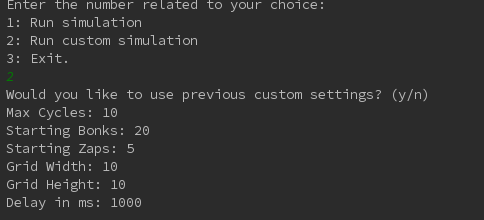
\includegraphics[width=15cm]{test2}
As you can see the settings are identical to those I entered in the first test. This is the result I expected as I am using java properties to save and load these settings.

\subsection{Test 3}
This test was done to show that the game ends when all bonks are killed. To ensure this happened I set an equal number of zaps to bonks to start with.\\
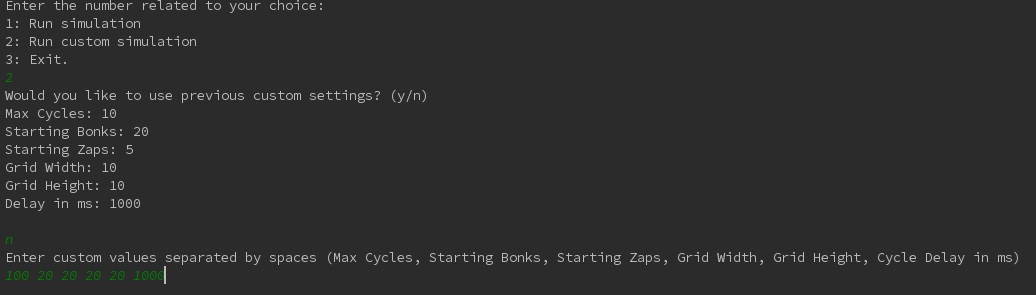
\includegraphics[width=15cm]{test3a}
I ran the 'game' with these settings.\\
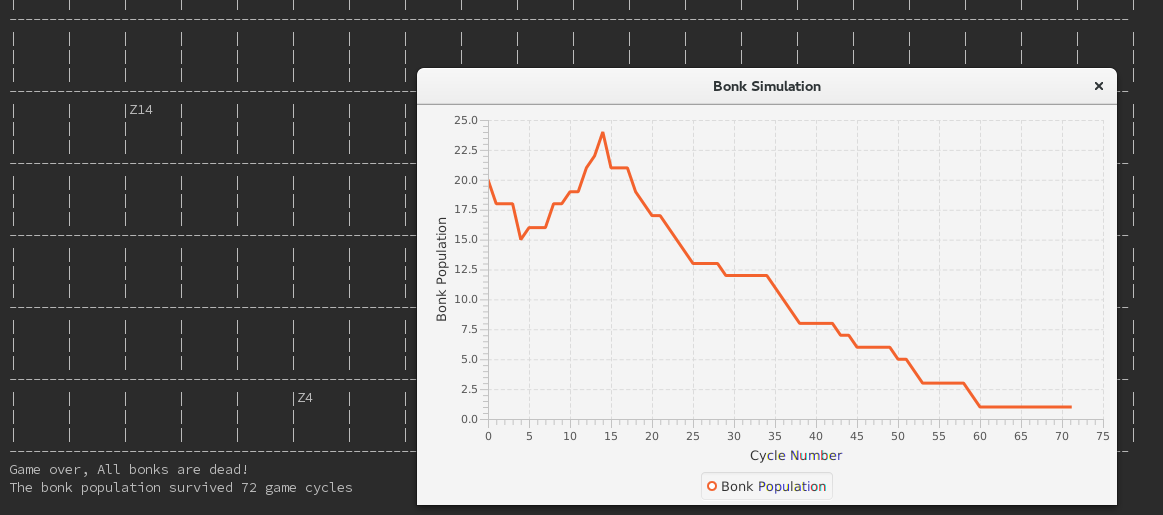
\includegraphics[width=15cm]{test3b}
As the image above shows, the 'game' successfully ends when all bonks are killed and in this example it took 72 game cycles. You can see the progression of the bonks dying on the graph on the right.\\ 
One issue I have noticed here is that the graph shows the bonk populations up until n-1 cycles in the case that all bonks are killed and therefore the graph never declines to 0. This could be an issue with my endGame() function.

\subsection{Test 4}
This is a simple test to ensure that the program closes when you enter 3 on the main menu.\\
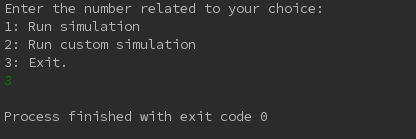
\includegraphics[width=15cm]{test4}

\subsection{Test 5}
This is a test aimed at the random positioning of beings at the start of a 'game'. Below are two images of two seperate times running the game on the first cycle.\\
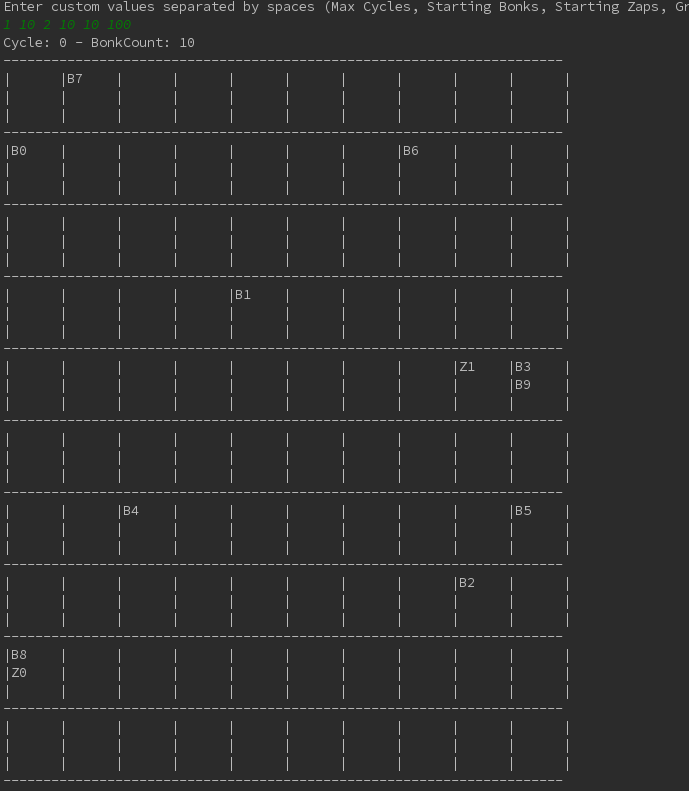
\includegraphics[height=7cm]{test5a}
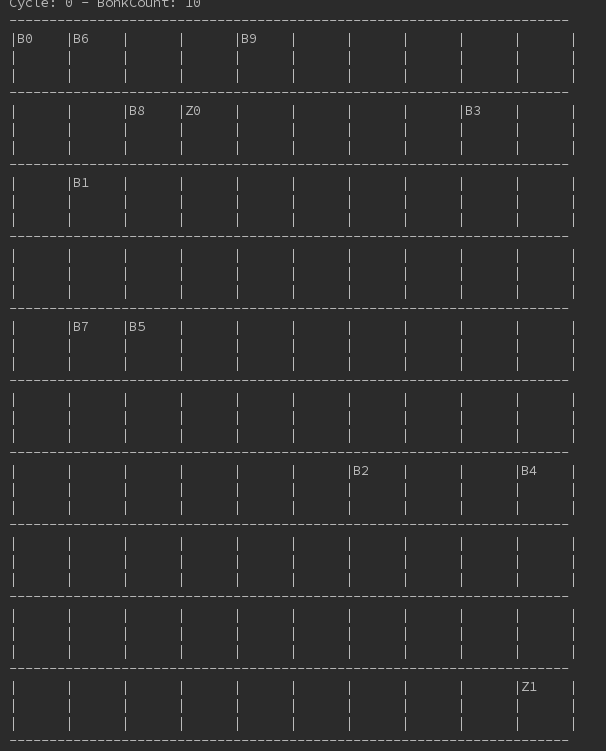
\includegraphics[height=7cm]{test5b}
 The two grids have completely different positionings of beings throughout the grid. This is what was expected due to the random nature of the 'game'.

\subsection{Test 6}
This test was supposed to check that the game can handle extremes. To test this I set the starting bonks to 3 million which is larger than the size of an integer. I used a long for my productionCount value within the bonk class so I did not expect this to be an issue.\\
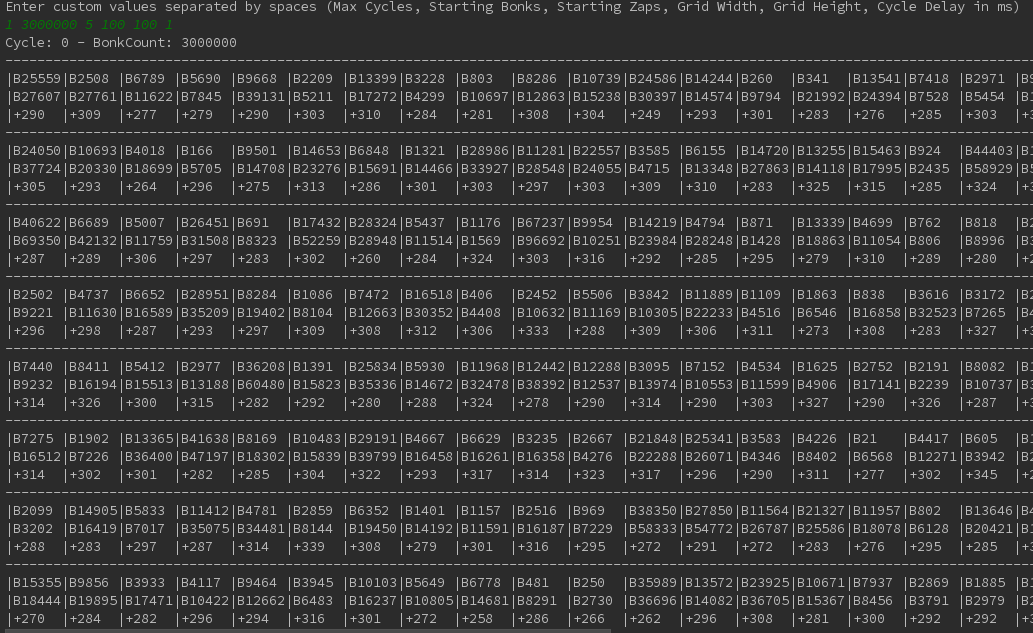
\includegraphics[width=15cm]{test6}
As you can see, the 'game' handles this fine and fills the world with bonks, despite the image not being able to show the entire grid world it shows enough to prove that the 'game' operates to expected levels.

\section{Evaluation}
	Throughout my project I ran into a few issues, the main problem was the time constraint placed and how many different ideas I had flair. If I were to do the assignment again I would focus on managing my time better to complete more of these flair ideas. I would give myself 80\% for this assignment as I feel my flair could do with a little more. On the other hand, I feel like my bonk population statistics idea worked really well and sets my assignment apart from others; the code behind it wasn't too complicated however using JavaFX was new to me and I ran into a few issues when trying to implement the idea. The general implementation of the assignment went really well and I feel like I have successfully implemented all of the features required by the brief. I opted not to implement the grid world in JavaFX as this would have taken up more of my time and I wanted to make sure I put enough time into my write-up after the mini-assignment where I lost most of my marks there; however I feel that my implementation of grid world in a terminal environment looks quite nice and is very simplistic.  


\end{document}
